\documentclass[tikz, border=10 mm]{standalone}
\usetikzlibrary{calc,angles,quotes,arrows.meta}
\begin{document}
	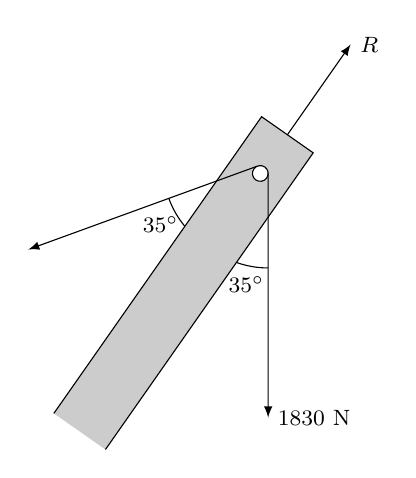
\begin{tikzpicture}[>=latex,,scale=2,font=\footnotesize]
		\def\r{0.05cm}%bán kính ốc
		\def\goc{35}
		\begin{scope}[rotate=-\goc]
			\coordinate (O) at (0,0);
			\coordinate (A) at (180-\goc:\r);
			\coordinate (B) at (\goc:\r);
			\coordinate[rotate around={-90:(A)}] (A') at ($(O)!-30!(A)$);
			\coordinate[rotate around={90:(B)}] (B') at ($(O)!-30!(B)$);
			\coordinate (M) at (-0.5,-2);
			\pic[draw,angle eccentricity=1.2,angle radius=1.2cm,"{${\goc}^\circ$}"] {angle=A'--A--M};
			\coordinate (N) at (0.5,-2);
			\pic[draw,angle eccentricity=1.2,angle radius=1.2cm,"{${\goc}^\circ$}"] {angle=N--B--B'};
			\draw[->] (0,0.15)--(0,1)node[right]{$R$};
			\draw[fill=gray!40] (0.2,-2)--(0.2,0.3)--(-0.2,0.3)--(-0.2,-2);
			\draw[fill=white] (O) circle (\r);
			\draw[<-] (A')--(A);
			\draw[<-] (B')node[right]{$1830$ N}--(B);
		\end{scope}
	\end{tikzpicture}
\end{document}